Here you can see how to include an image in your document.

\begin{sidewaysfigure}
\centering
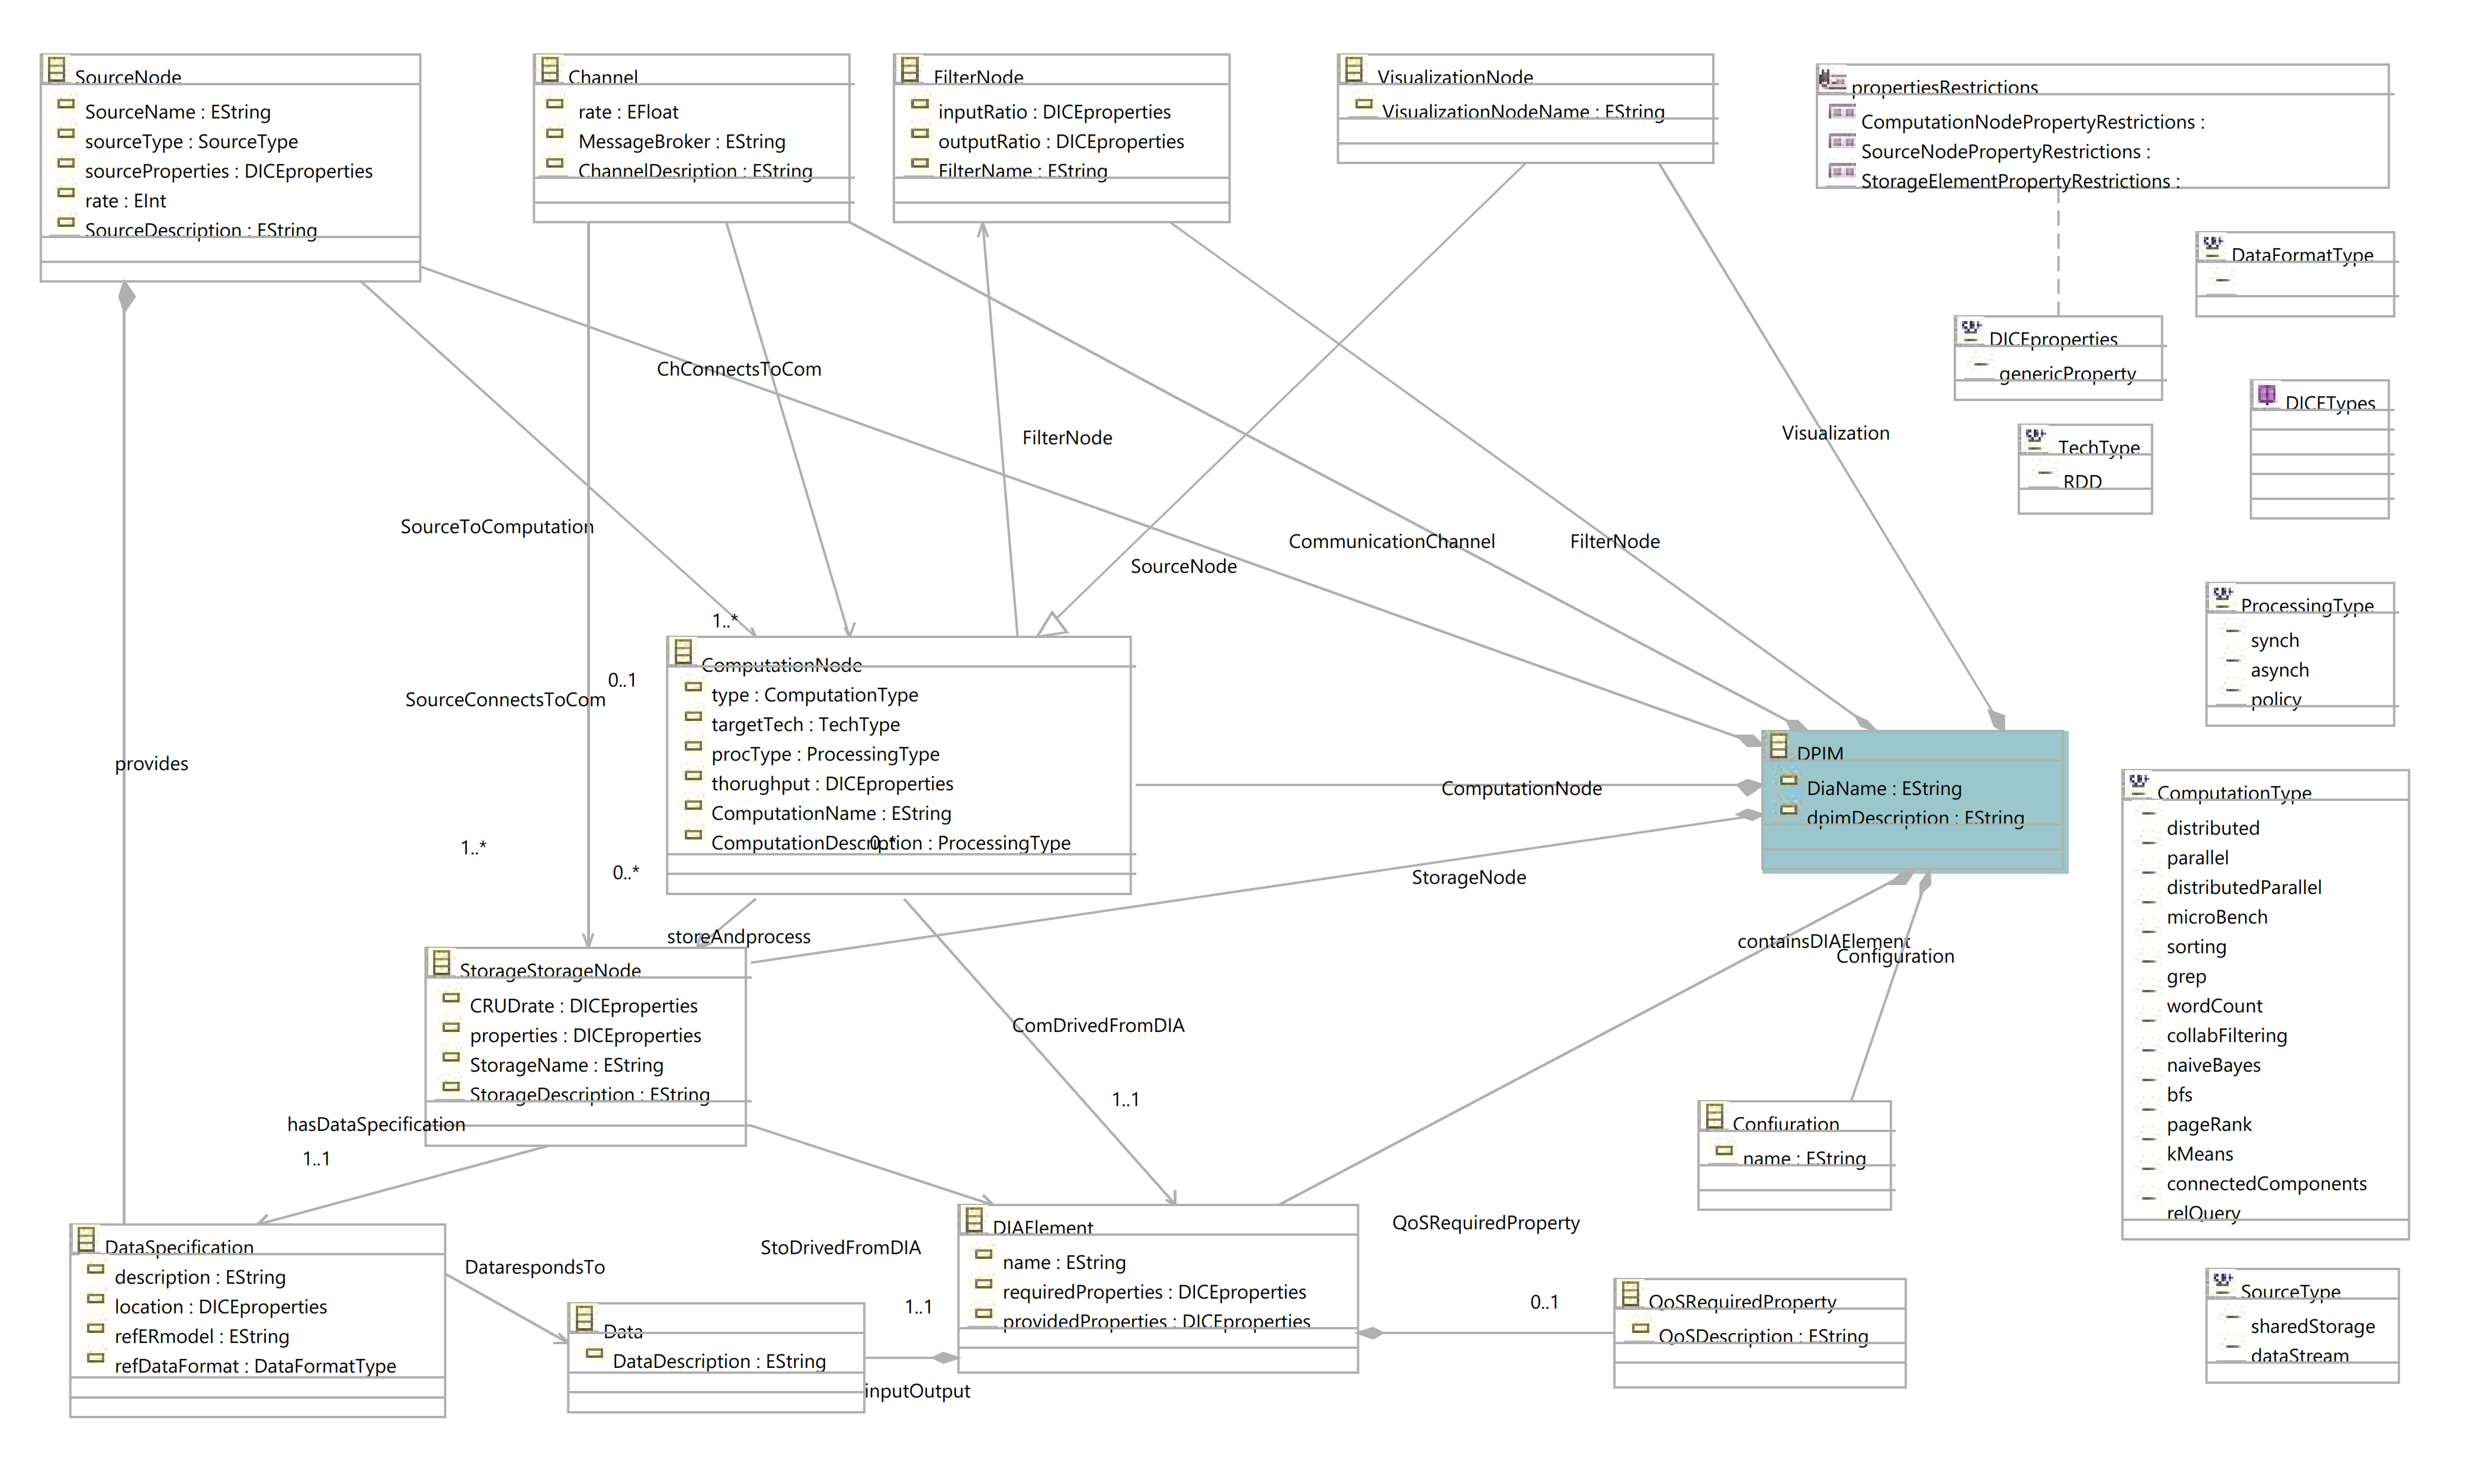
\includegraphics[width=\textwidth]{Images/11.png}
\caption{\label{fig:metamodel}DICE DPIM metamodel.}
\end{sidewaysfigure}

\begin{figure}
\centering
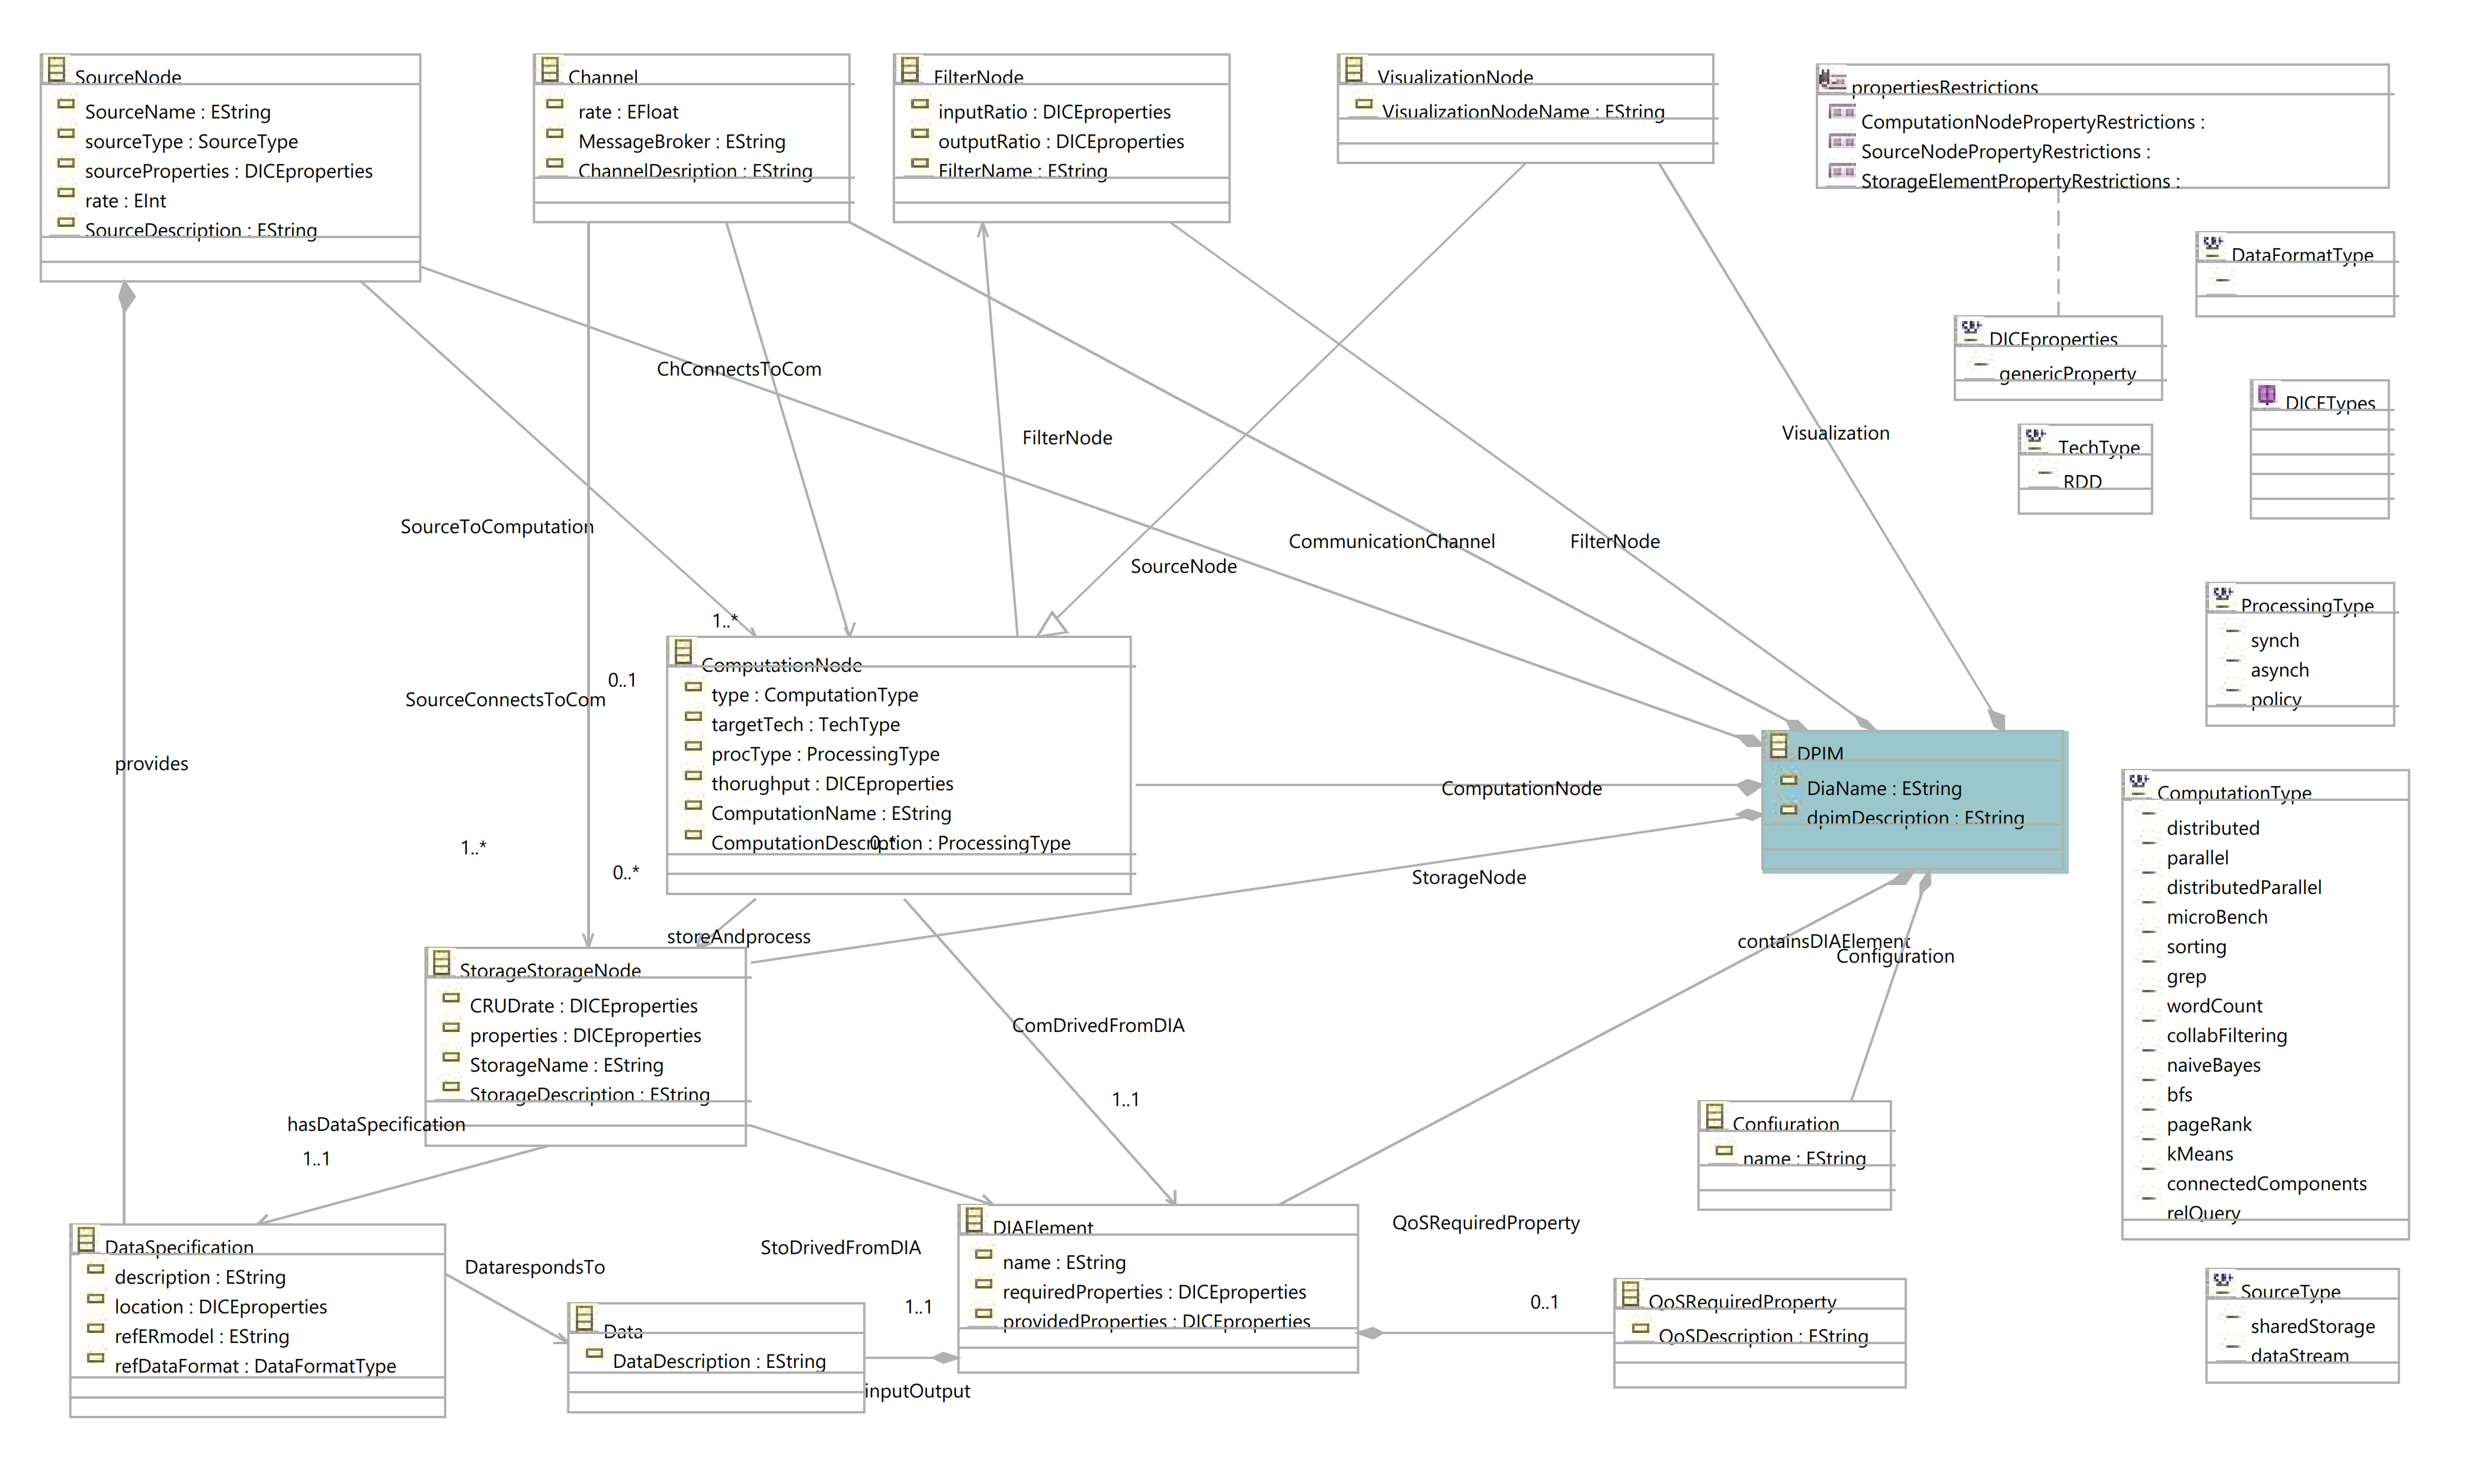
\includegraphics[width=\textwidth]{Images/11.png}
\caption{\label{fig:metamodel2}DICE DPIM metamodel in portrait form.}
\end{figure}

Here is the command to refer to another element (section, figure, table, ...) in the document: \emph{As discussed in Section~\ref{sect:overview} and as shown in Figure~\ref{fig:metamodel}, ...}. Here is how to introduce a bibliographic citation~\cite{DAM}. Bibliographic references should be included in a \texttt{.bib} file. 

Table generation is a bit complicated in Latex. You will soon become proficient, but to start you can rely on tools or external services. See for instance this \href{https://www.tablesgenerator.com}{https://www.tablesgenerator.com}. 

\subsection{Product perspective}
\subsection{Product functions}
the product will be used by farmers, policy makers and agronomists
\subsection{User characteristics}
\subsection{Assumptions, dependencies and constraints}
Assumptions TODO :
\begin{itemize}
	\item
	Cropping seasons are the same on the whole Telengana State and follow the Kharif/Rabi calendar (see Recommended System of Breeder Seed Indent and Supply)
\end{itemize}
\subsubsection{Domain Properties}
here are some domain properties/assumptions
\begin{itemize}
	\item
	DP1 : Every farmer has a smartphone (with geo-tracking,... properties)
	\item
	DP2 : Soil moisture data are updated every 2 days
	\item
	DP : Rainfall conditions are daily updated
	\item
	DP : Rainfall previsions (24/48/72h) are daily updated
	\item
	DP : Data fetched on the different governmental sites are trustworthy reliable
	\item
	DP3 : Farmers are fair when providing data, suggestions and problems
	\item
	DP4 : There are at least 2 farmers and 1 policy maker
	\item
	DP5 : Data from sensors are accurate (in a ... extent)
	\item
	DP6 : Data from the Web are accurate (in a ... extent)
	\item
	DP7 : Sensors are always available, or at least, there is a sufficient number of them to properly describe an area (precision of the DP ?)
	\item
	DP8 : farmers should have received credentials to log in the application
	
\end{itemize}

\subsubsection{use cases}
Here is the diagram for farmers. We suppose they are logged in the application. In case they are not they can simply log in or create an account and then log in.
\begin{figure}
	\centering
	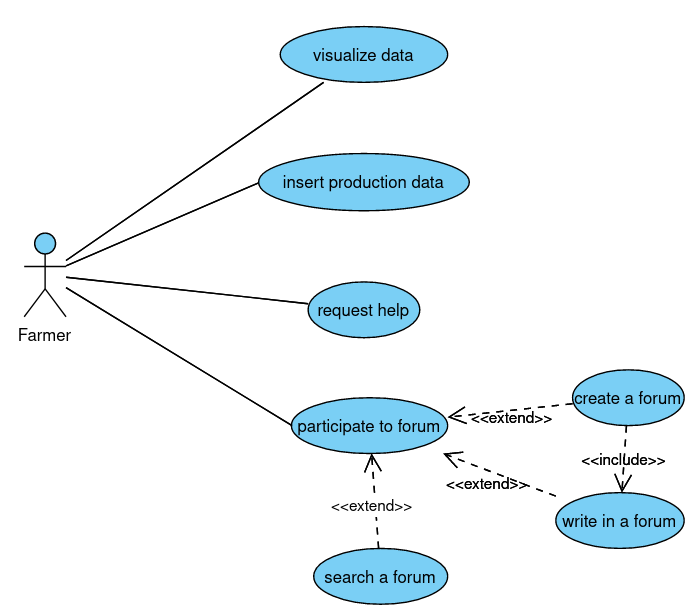
\includegraphics[width=\textwidth]{Images/use-case-farmer.png}
	\caption{\label{fig:usecasefarmer}Use case diagram for logged in farmer}
\end{figure}

\begin{figure}
	\centering
	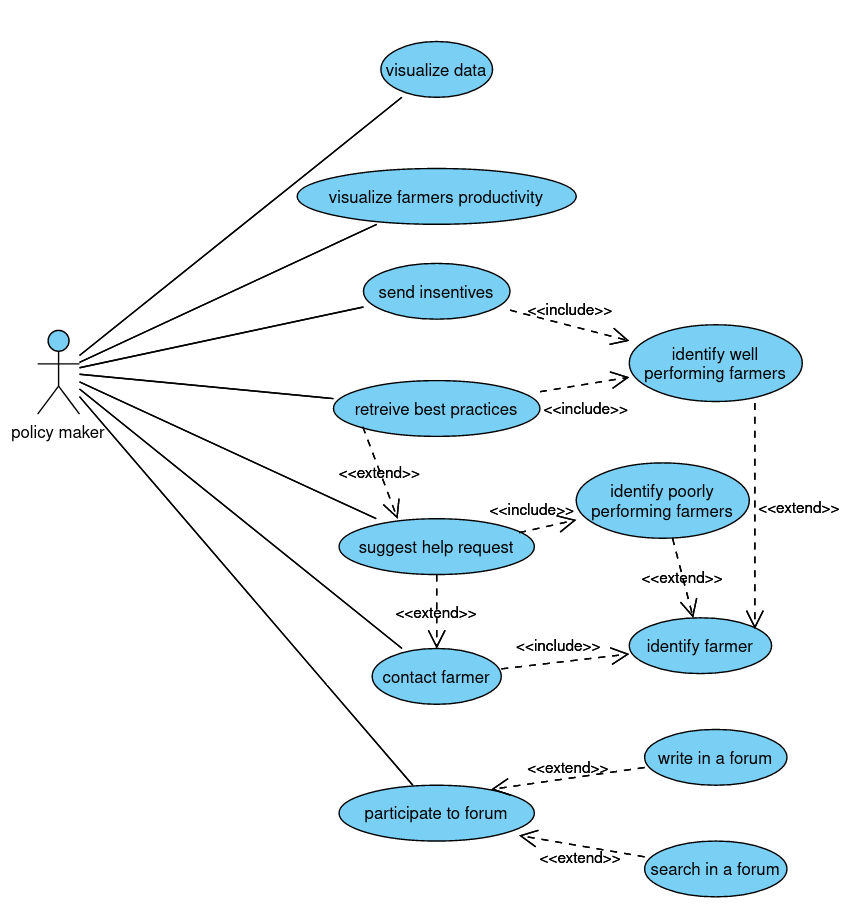
\includegraphics[width=\textwidth]{Images/use-case-policy.png}
	\caption{\label{fig:usecasepolicymakers}Use case diagram for logged in policy makers}
\end{figure}
